% !TeX root = ../main.tex
\documentclass[./../main.tex]{subfiles}

\begin{document}

Phần này mô tả lại 3 luồng hoạt động chính bao gồm luồng đăng nhập, luồng sử dụng của quản trị viên Khoa và luồng hoạt động của quản trị viên hệ thống.

\subsection{Luồng đăng nhập}

Người dùng điền thông tin tài khoản và mật khẩu, hoặc lựa chọn đăng nhập
bằng Google để đăng nhập vào hệ thống. Hệ thống sẽ dựa vào vai trò của
người dùng là sinh viên, giảng viên, đối tác hay quản trị viên để điều
hướng người dùng tới trang phù hợp.

Hình \ref{fig:login_page} mô tả màn hình đăng nhập của hệ thống.

\begin{figure}[]
	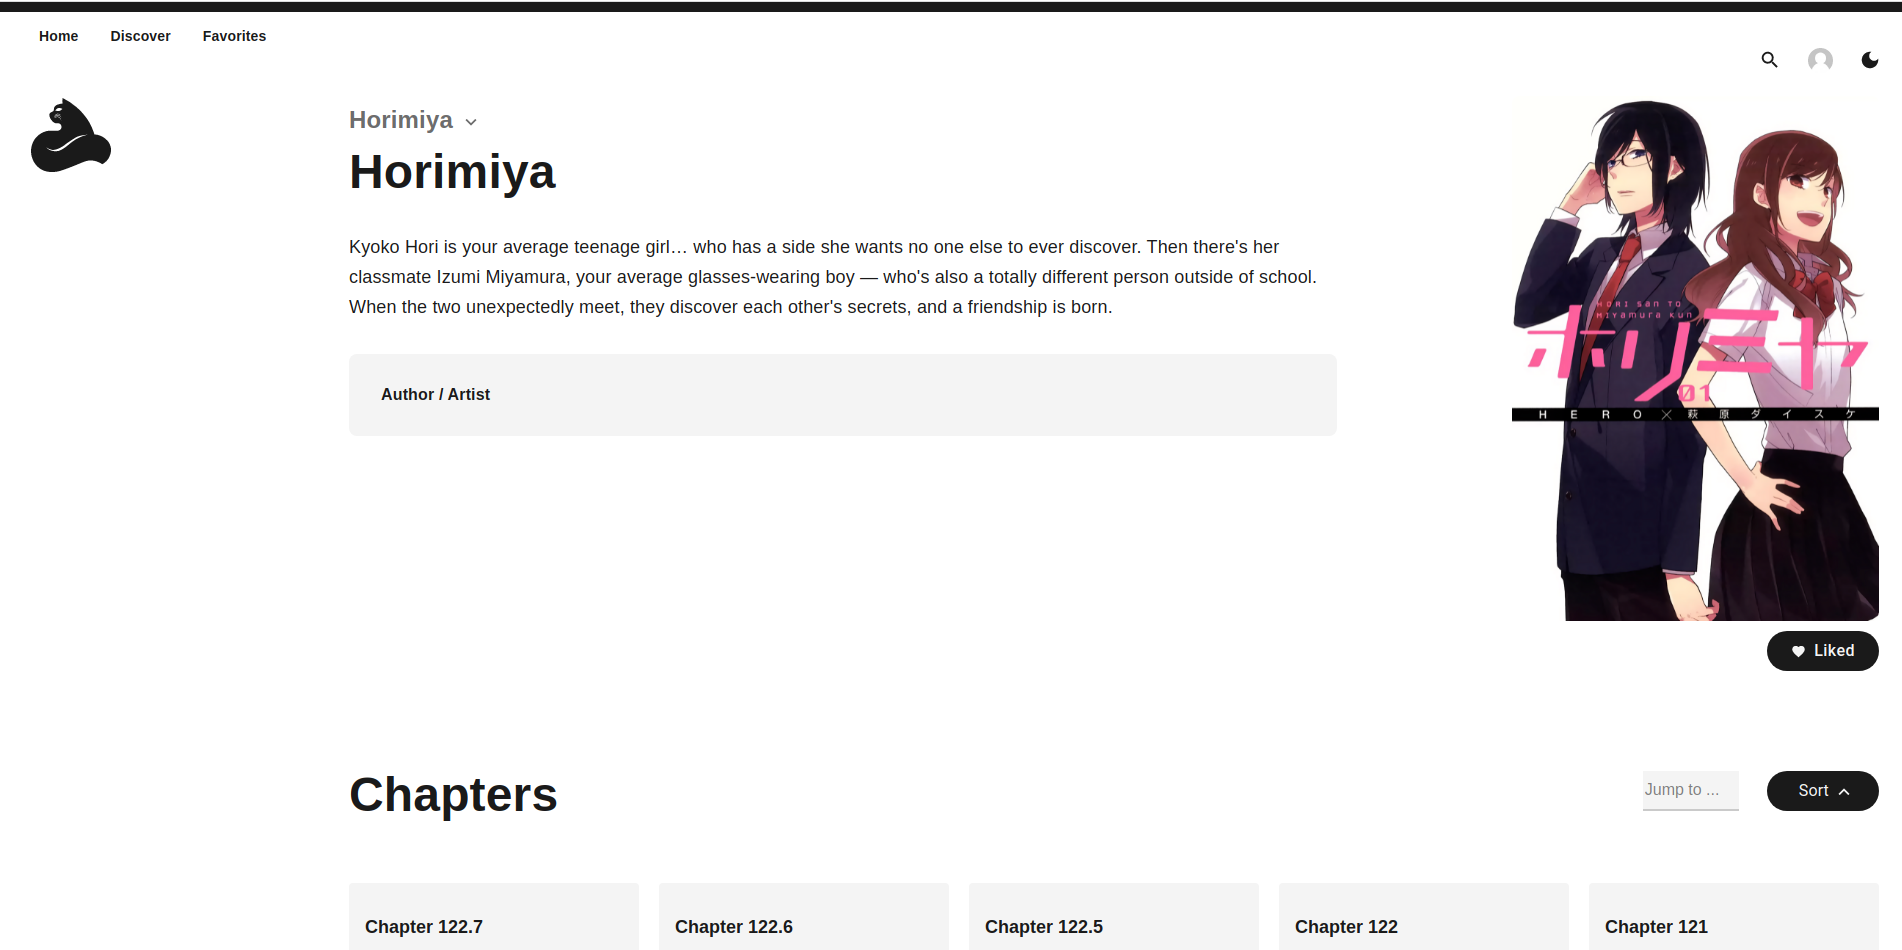
\includegraphics[width=\linewidth]{./images/image5.png}
	\caption{Luồng hình đăng nhập}
	\label{fig:login_page}
\end{figure}

\subsection{Luồng sử dụng của quản trị viên Khoa}

\paragraph*{Tạo kỳ thực tập mới}

Quản trị viên Khoa tạo một kỳ thực tập mới, các thông tin bao gồm năm, kỳ, ngày bắt đầu, ngày kết thúc, ngày bắt đầu đăng ký, ngày kết thúc đăng ký.

Hình \ref{fig:add_term_page} mô tả màn hình tạo kỳ thực tập mới.

\begin{figure}[]
	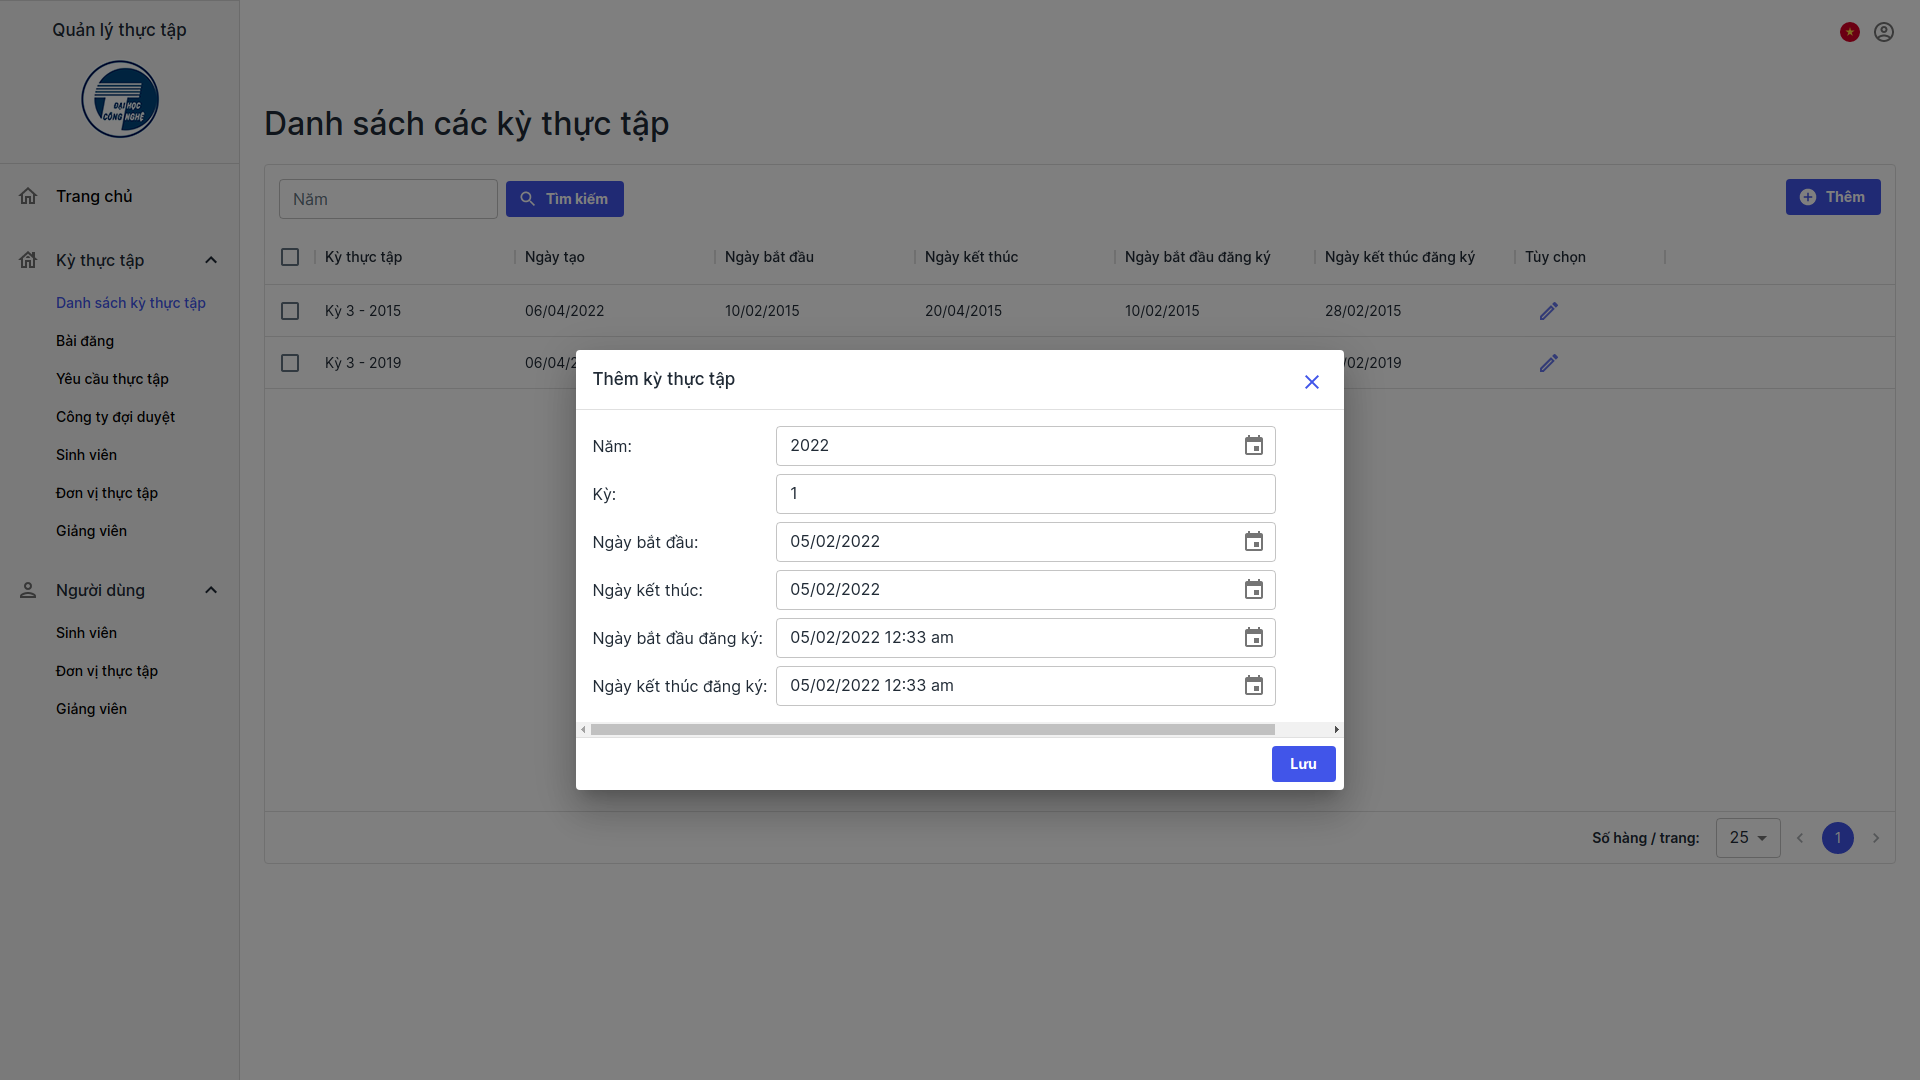
\includegraphics[width=\linewidth]{./images/image19.png}
	\caption{Màn hình tạo kỳ thực tập mới}
	\label{fig:add_term_page}
\end{figure}

\paragraph*{Tạo kỳ thực tập thành công}

Sau khi tạo thành công, hệ thống phản hồi lại thông báo và cập nhật danh sách các kỳ thực tập.

Hình \ref{fig:add_term_success} mô tả màn hình tạo kỳ thực tập mới thành công.

\begin{figure}[]
	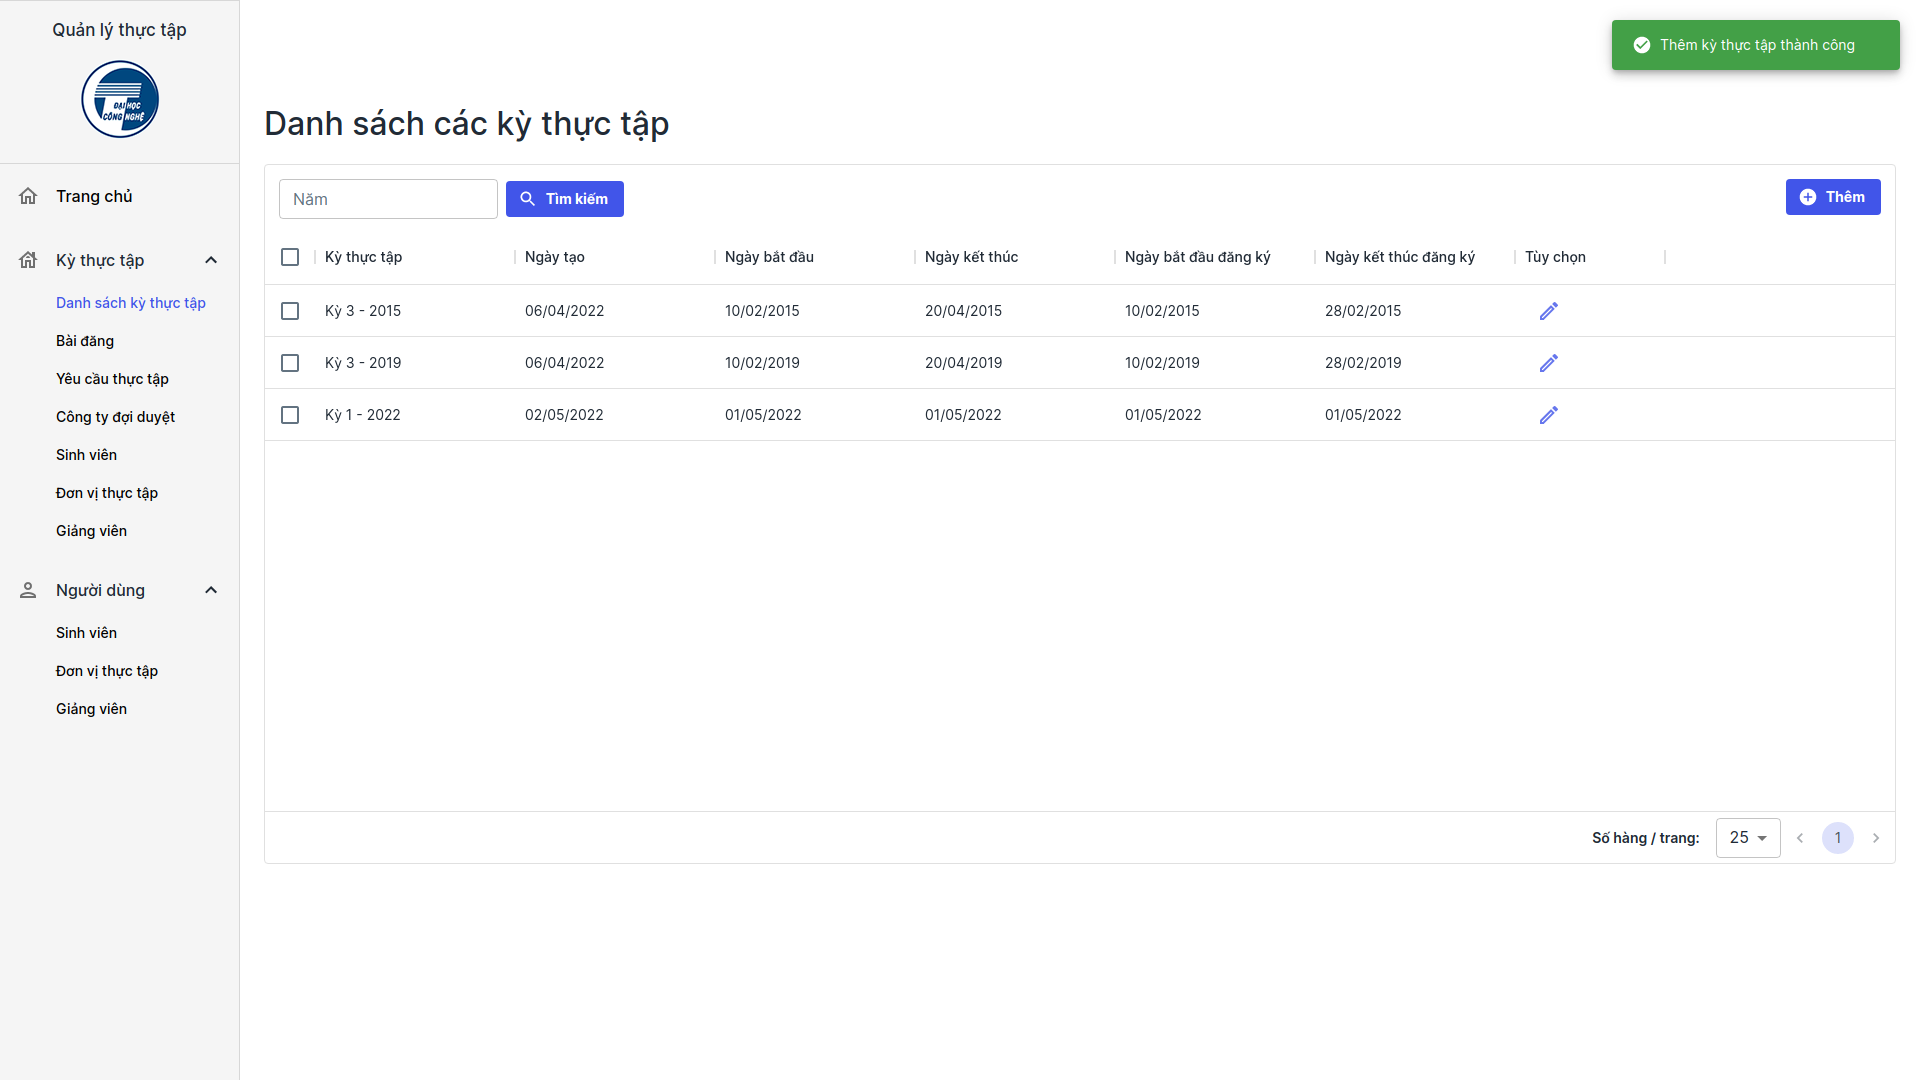
\includegraphics[width=\linewidth]{./images/image20.png}
	\caption{Màn hình tạo kỳ thực tập mới thành công}
	\label{fig:add_term_success}
\end{figure}

\paragraph*{Gán giảng viên cho sinh viên}

Sau khi sinh viên đã chốt nơi thực tập, quản trị viên chọn các sinh viên rồi thực hiện gán giảng viên.

Hình \ref{fig:assign_lecturer} mô tả màn hình gán giảng viên cho sinh viên.

\begin{figure}[]
	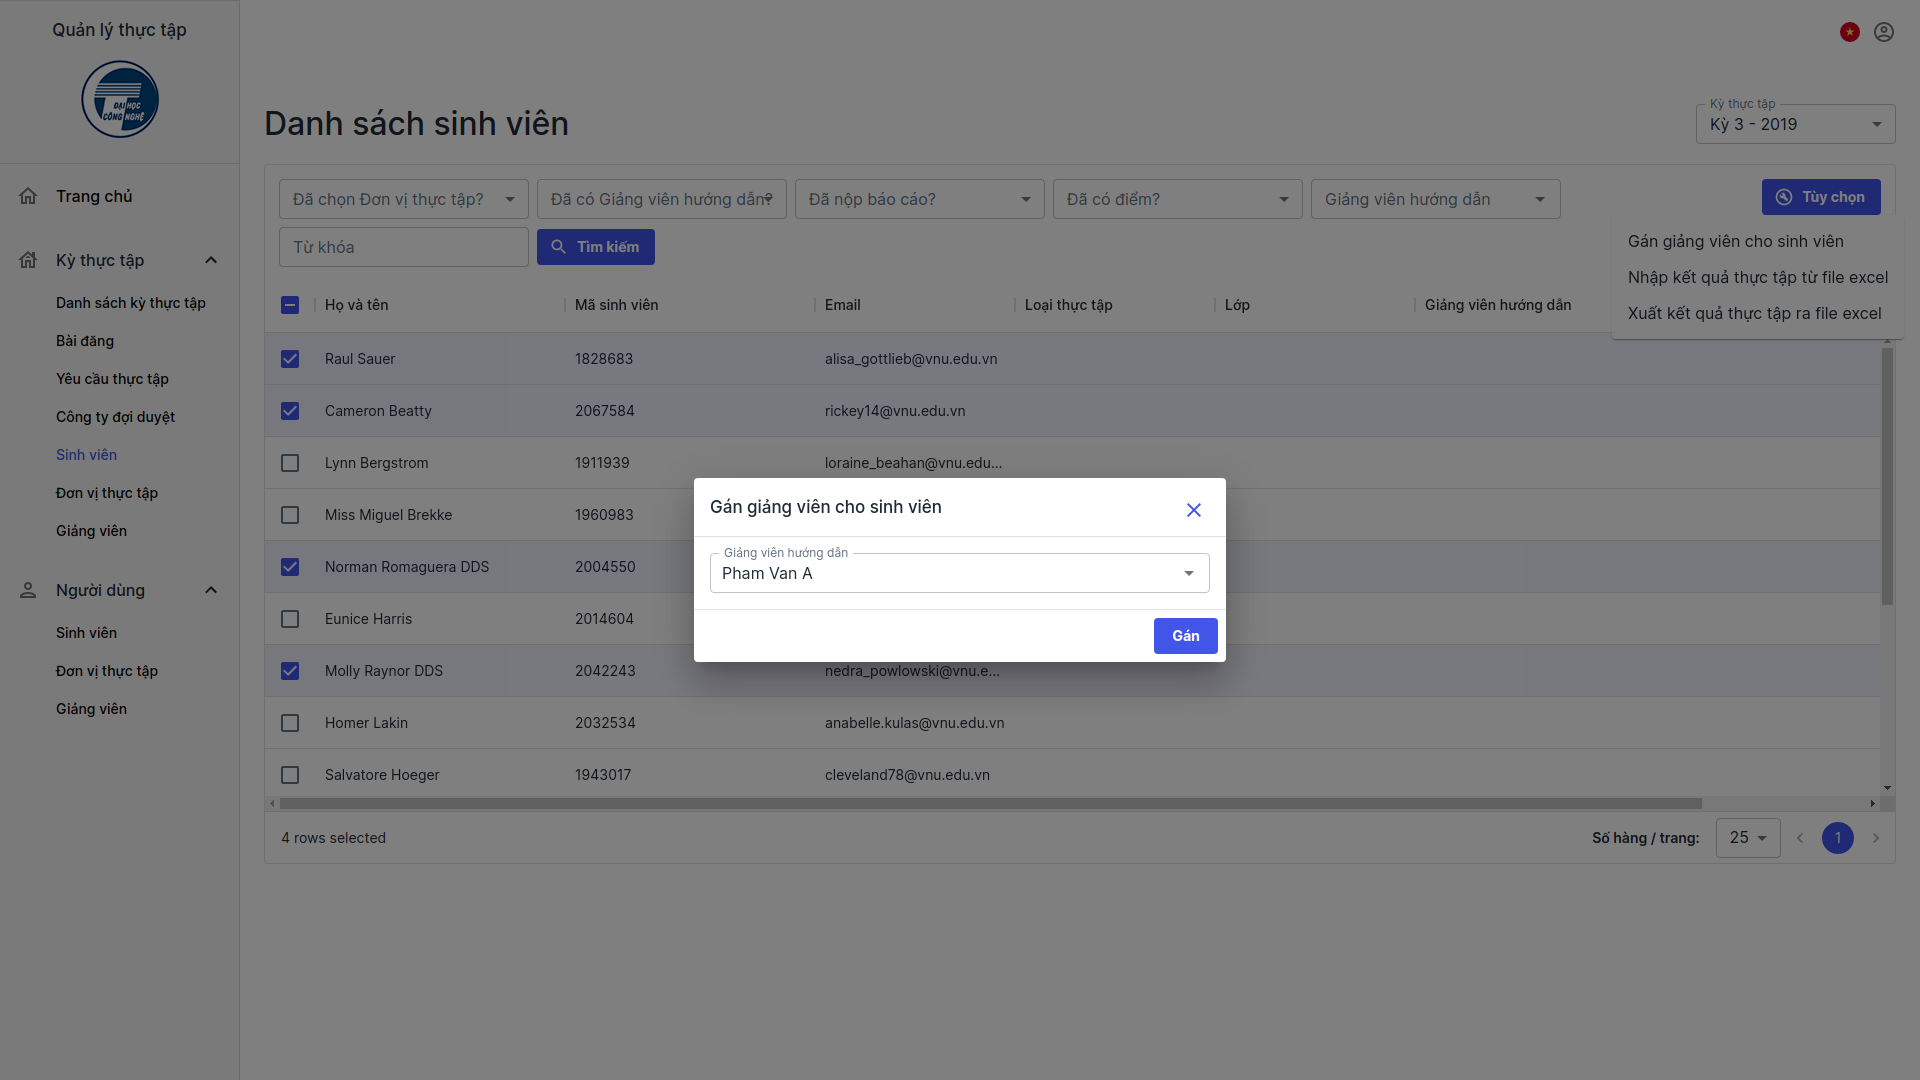
\includegraphics[width=\linewidth]{./images/image22.png}
	\caption{Màn hình gán giảng viên cho sinh viên}
	\label{fig:assign_lecturer}
\end{figure}

\paragraph*{Chấp nhận / Từ chối công ty}

Quản trị viên chọn một công ty đang ở chế độ Pending và thực hiện chấp nhận hay từ chối công ty.

Hình \ref{fig:reject_or_approve_company} mô tả màn hình Chấp nhận / Từ chối công ty.

\begin{figure}[]
	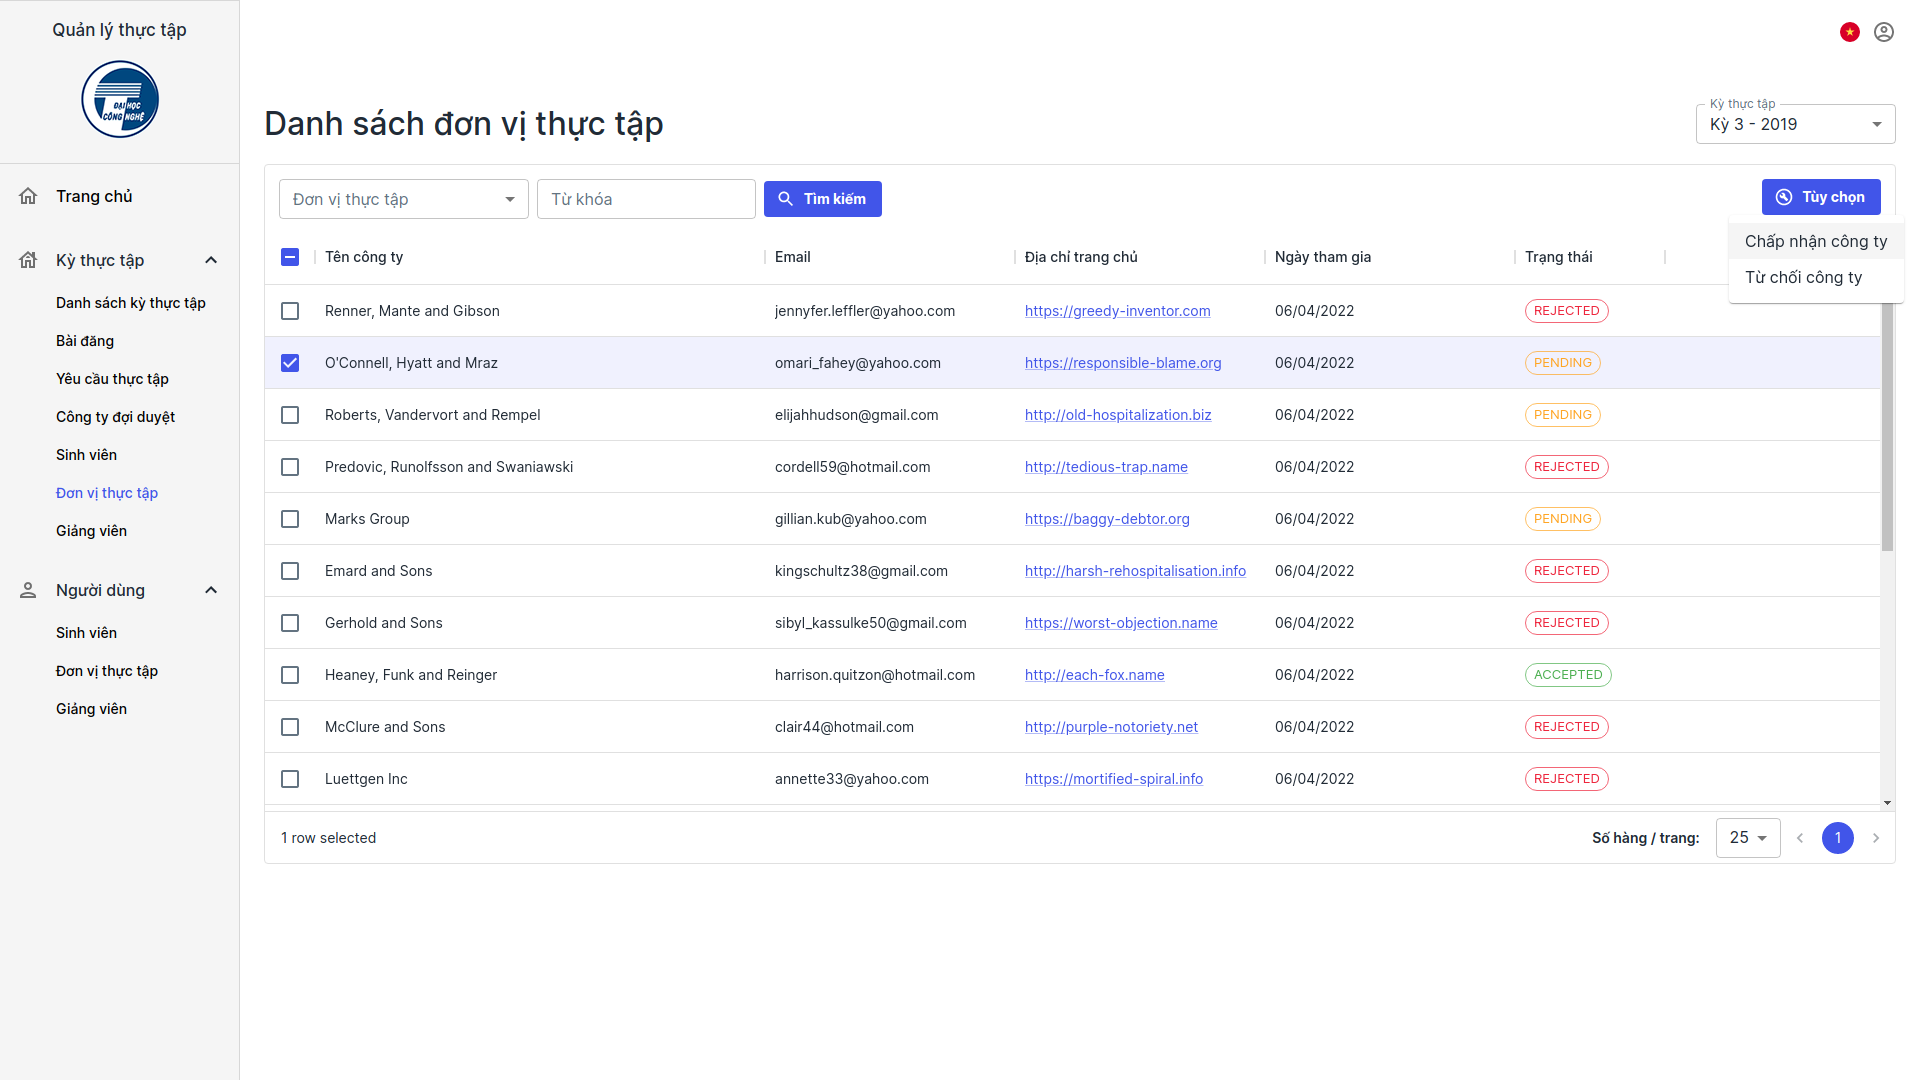
\includegraphics[width=\linewidth]{./images/image21.png}
	\caption{Màn hình Chấp nhận / Từ chối công ty}
	\label{fig:reject_or_approve_company}
\end{figure}

\subsection{Luồng sử dụng của quản trị viên hệ thống}

\paragraph*{Tạo Khoa mới}

Quản trị viên thực hiện tạo Khoa mới gồm có: tên khoa, email quản trị viên Khoa.

Hình \ref{fig:add_org} mô tả màn hình tạo Khoa mới.

\begin{figure}[]
	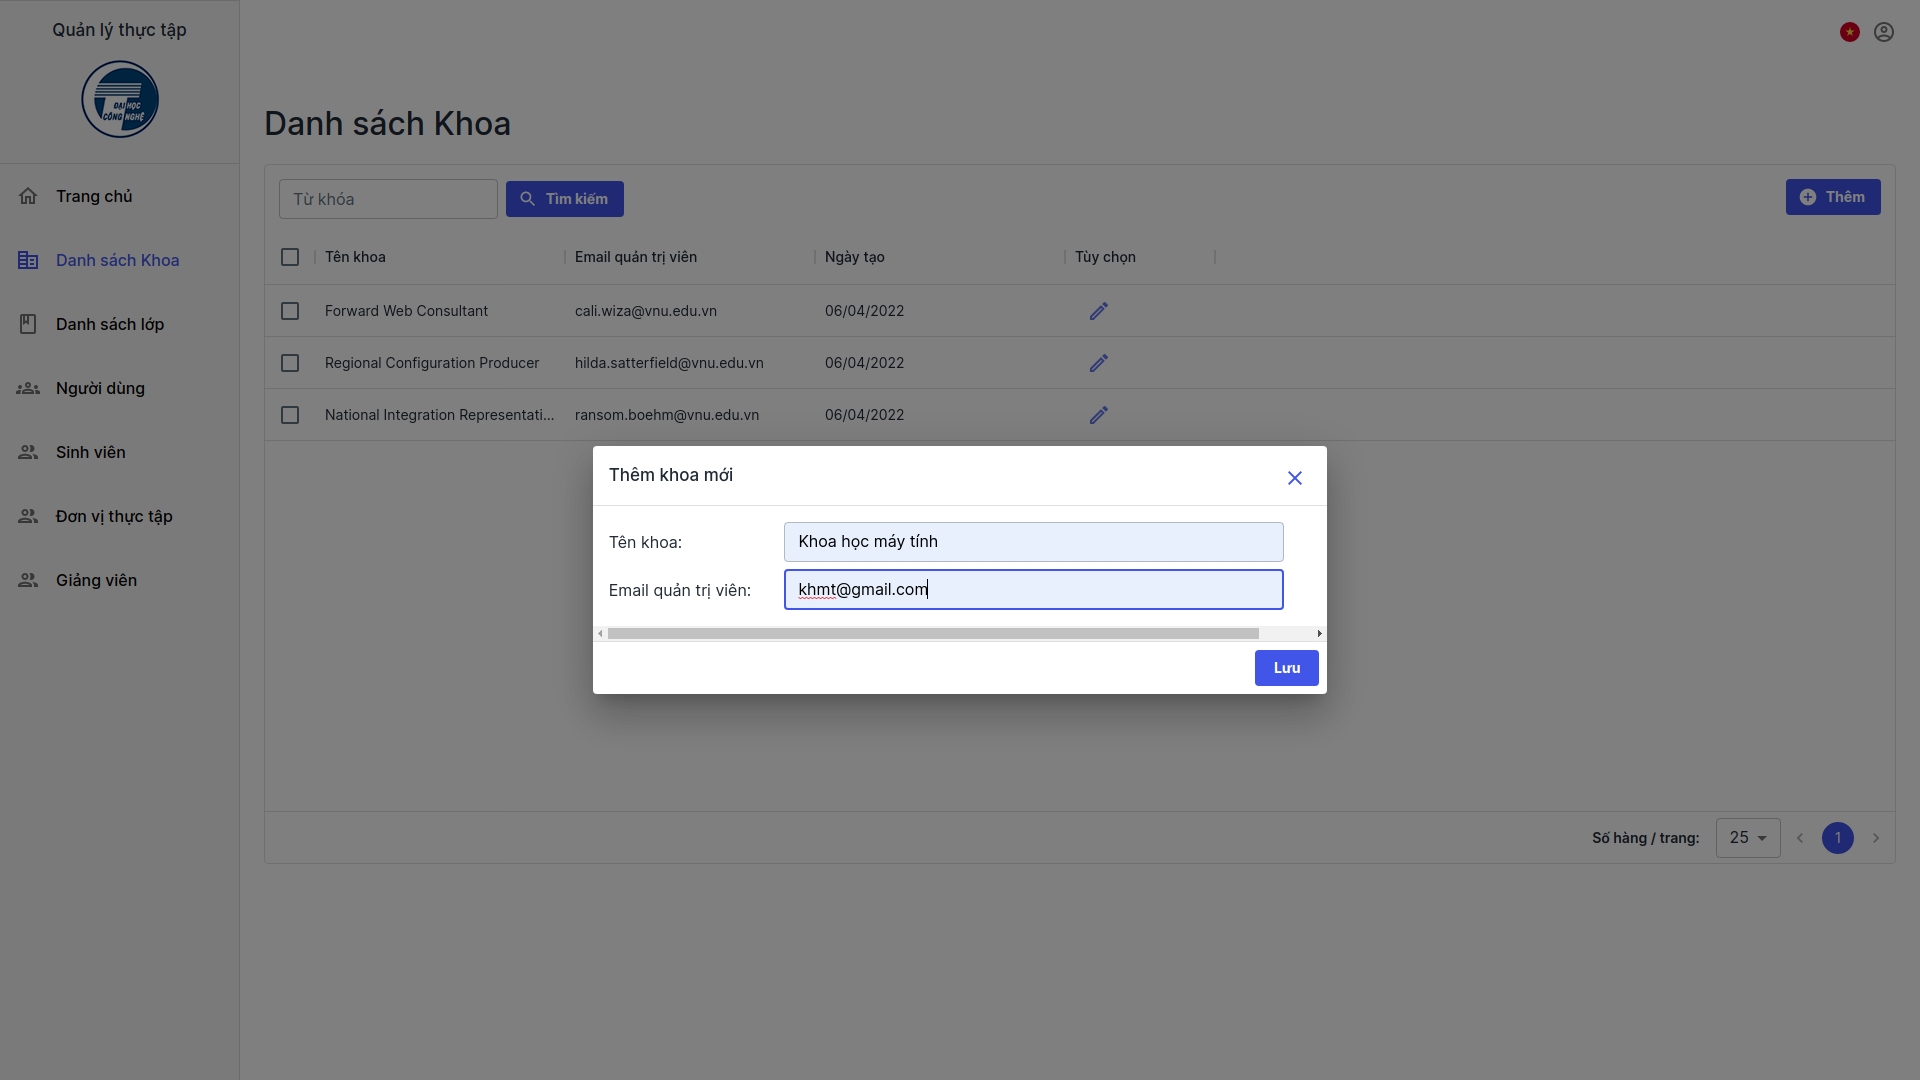
\includegraphics[width=\linewidth]{./images/image23.png}
	\caption{Màn hình tạo Khoa mới}
	\label{fig:add_org}
\end{figure}

\paragraph*{Tạo Khoa mới thành công}

Sau khi tạo thành công, một email được gửi đến hòm thư cung cấp mật khẩu cho quản trị viên Khoa.

% Hình \ref{fig:add_org_success} mô tả màn hình hòm thư sau khi tạo Khoa mới thành công.

\paragraph*{Tạo Lớp mới}

Quản trị viên thực hiện tạo lớp mới gồm các thông tin: tên lớp, chương trình giảng dạy.

Hình \ref{fig:add_class} mô tả màn hình tạo Lớp mới.

\begin{figure}[]
	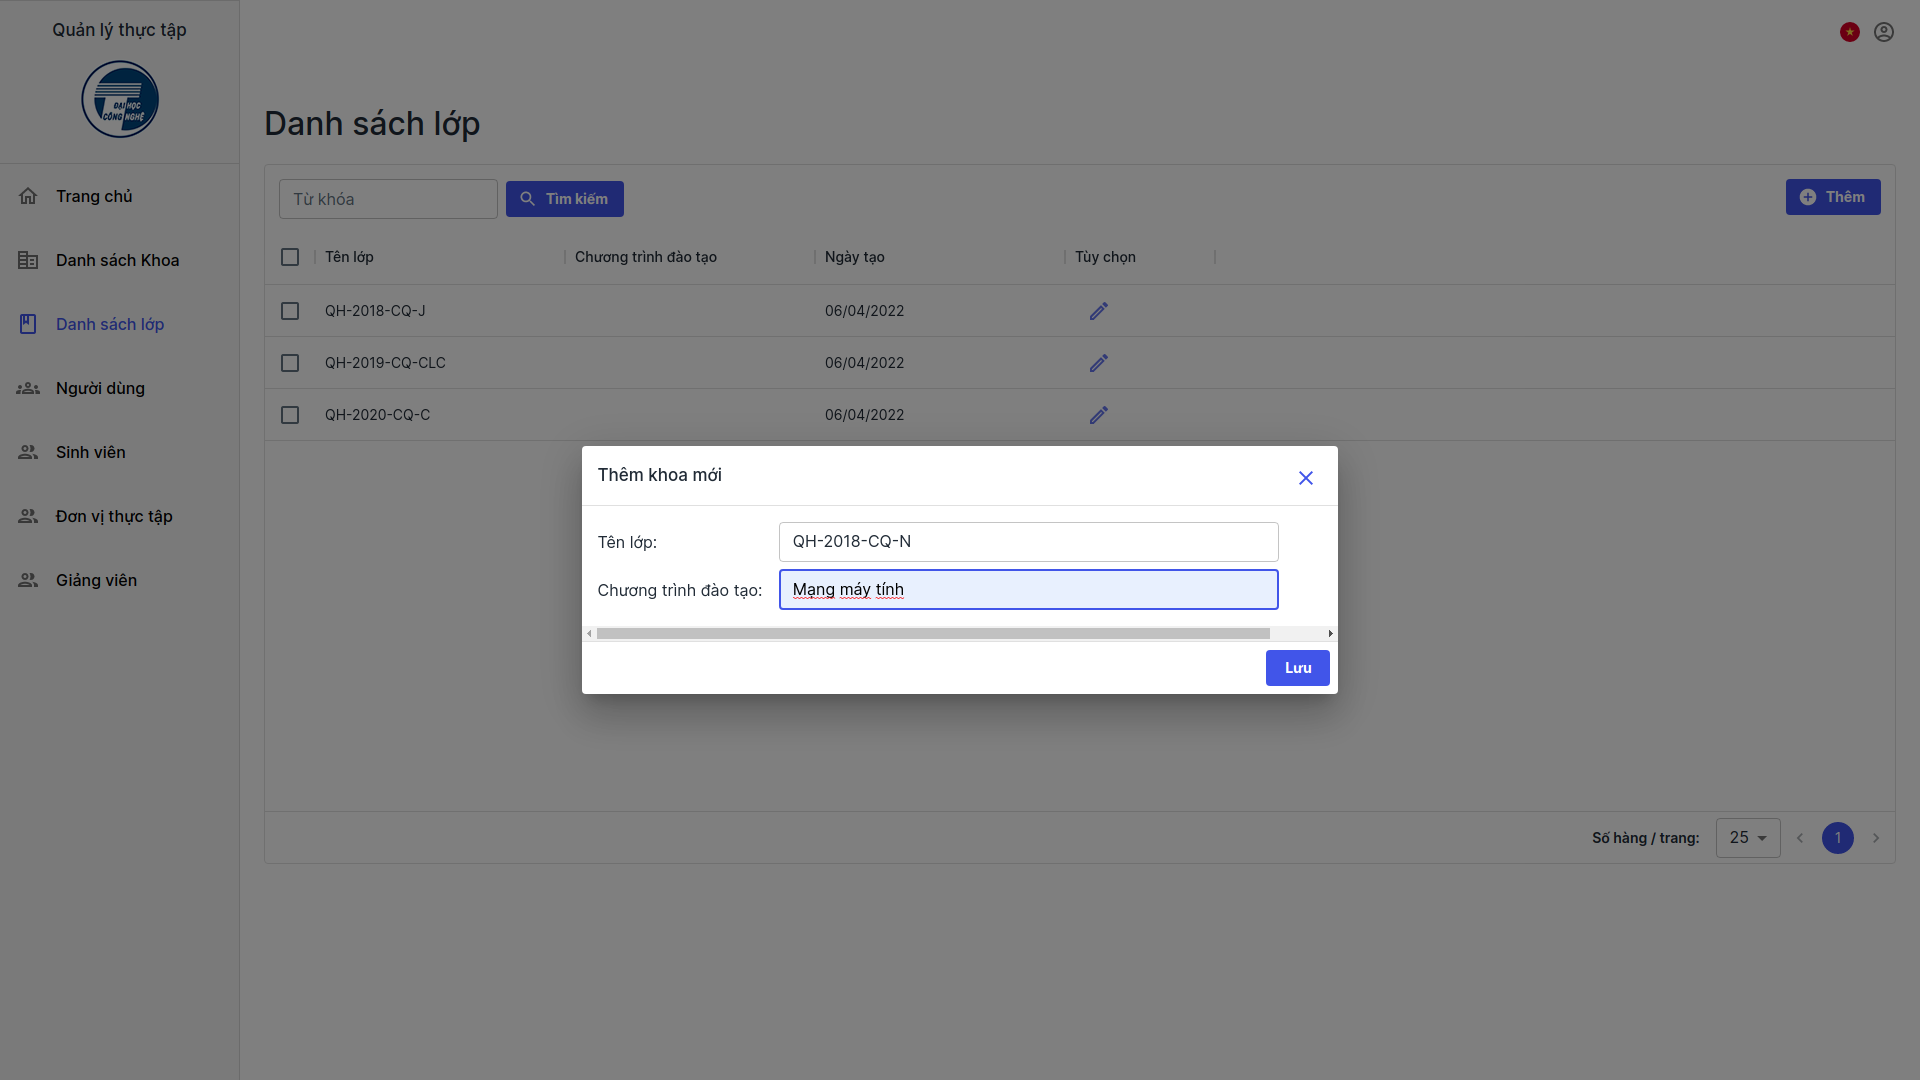
\includegraphics[width=\linewidth]{./images/image25.png}
	\caption{Màn hình tạo Lớp mới}
	\label{fig:add_class}
\end{figure}

\paragraph*{Nhập vào Danh sách sinh viên}

Từ màn hình Sinh viên, quản trị viên chọn chức năng Nhập danh sách từ file excel để tải lên danh sách sinh viên của hệ thống.

Hình \ref{fig:choose_file} mô tả màn hình chọn file Danh sách sinh viên.

\begin{figure}[]
	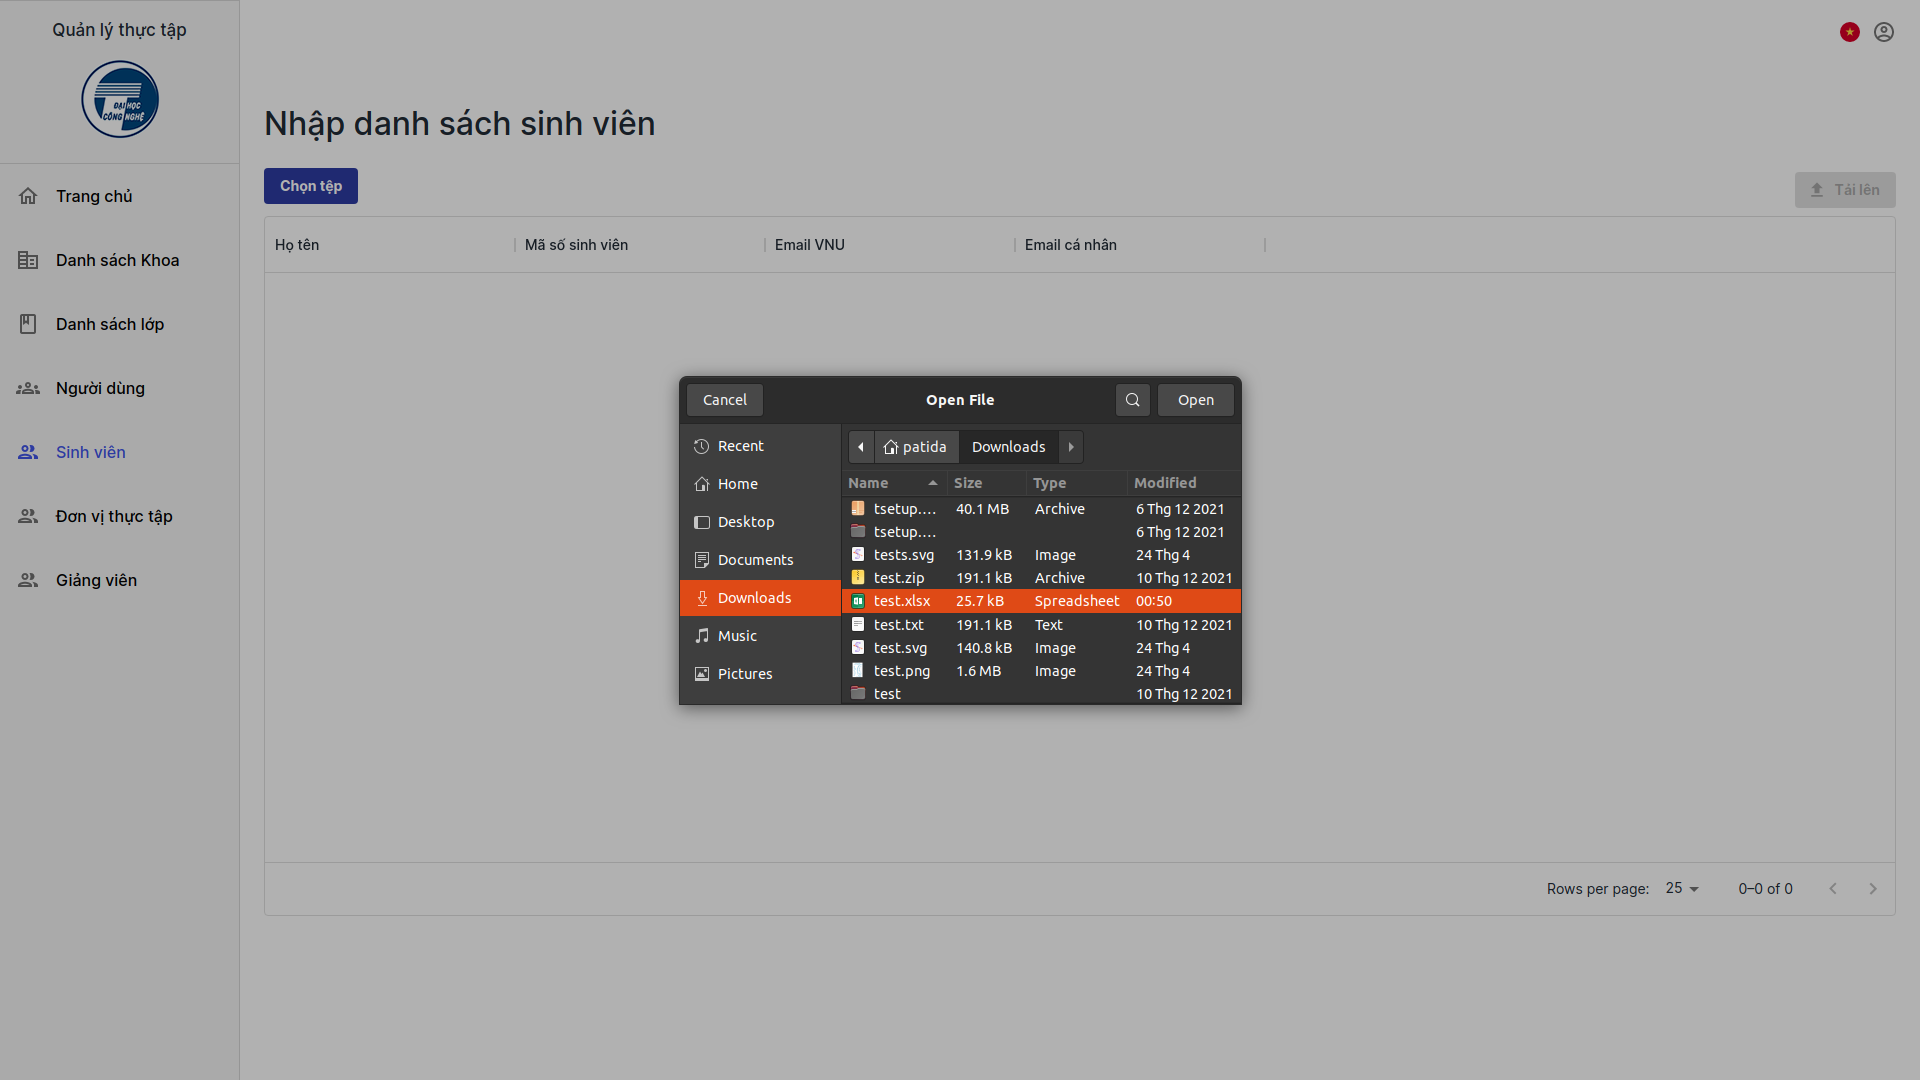
\includegraphics[width=\linewidth]{./images/image27.png}
	\caption{Màn hình chọn file Danh sách sinh viên}
	\label{fig:choose_file}
\end{figure}

Sau khi chọn xong tệp, dữ liệu ở trong file được hiển thị lại trên màn hình. Quản trị viên chọn chức năng Tải lên để tải lên danh sách sinh viên.

Hình \ref{fig:upload_list} mô tả màn hình tải lên file Danh sách sinh viên.

\begin{figure}[]
	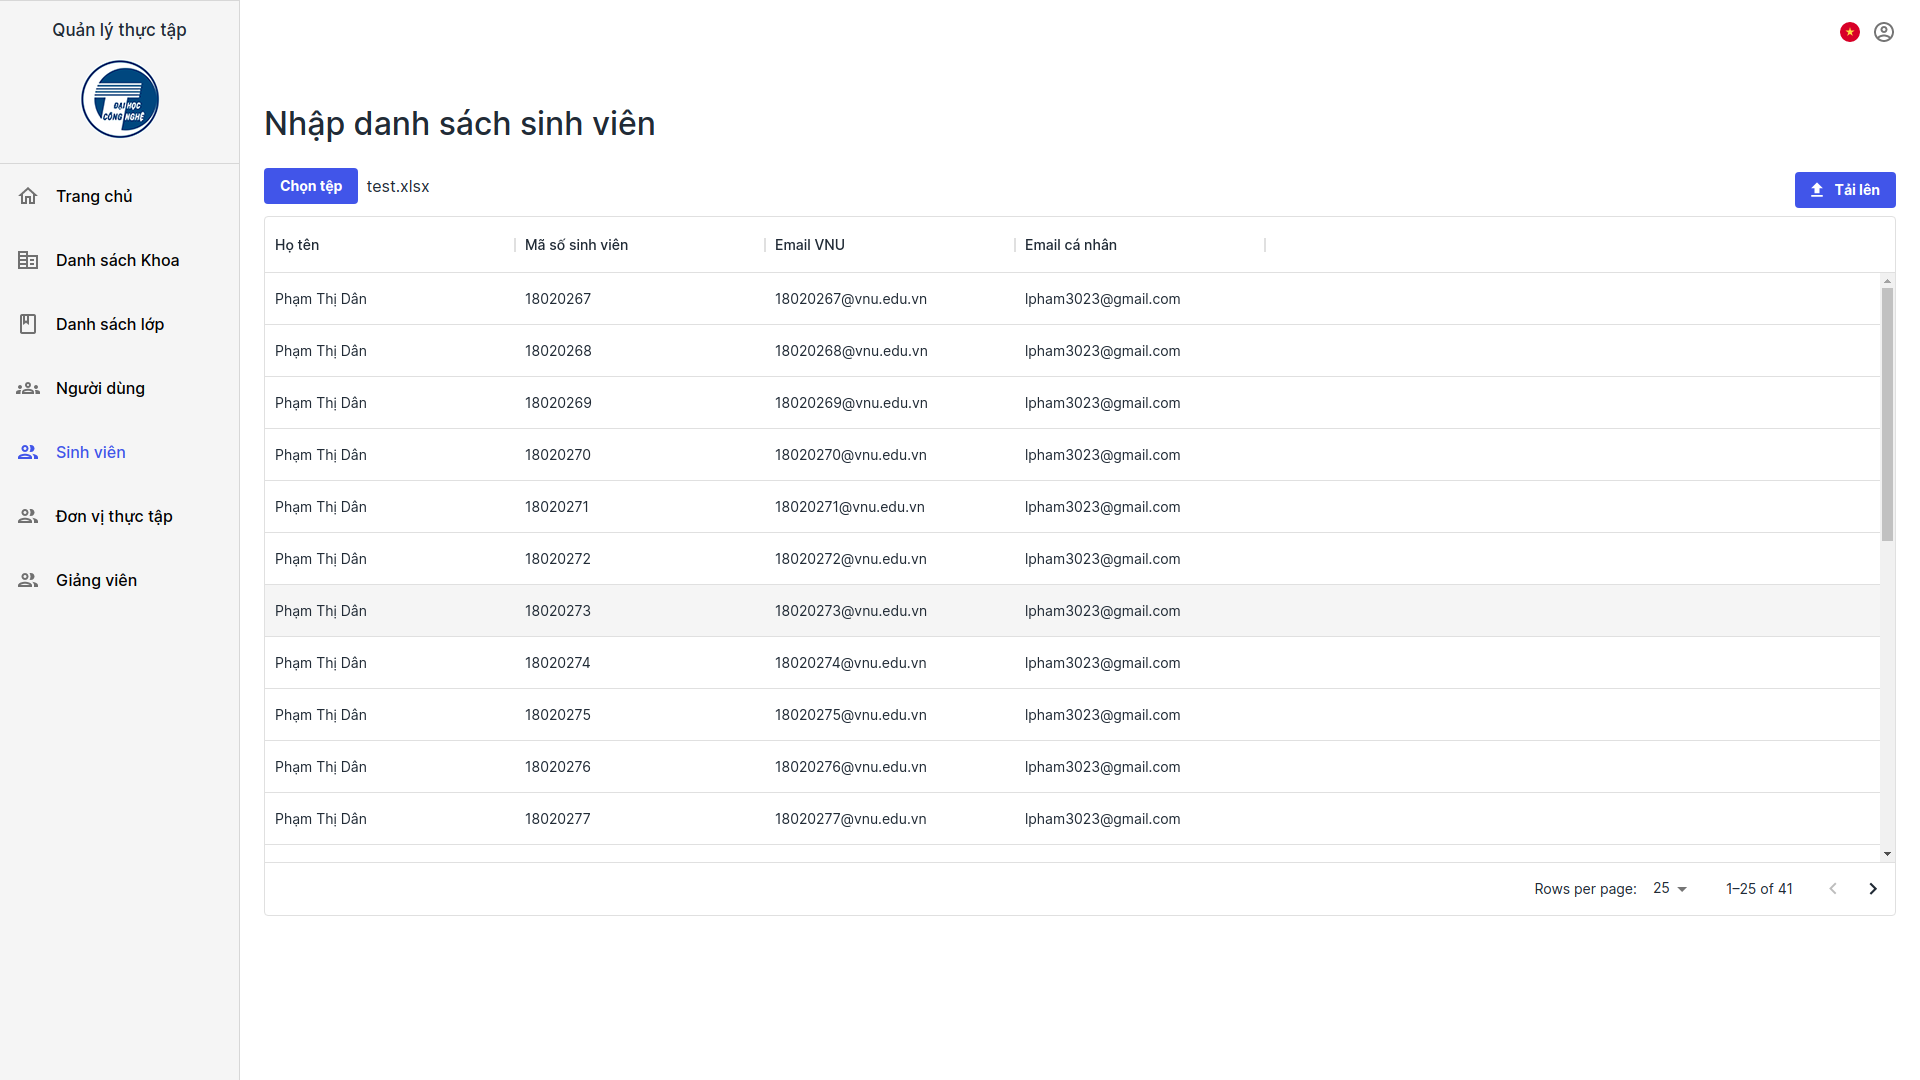
\includegraphics[width=\linewidth]{./images/image28.png}
	\caption{Màn hình tải lên file Danh sách sinh viên}
	\label{fig:upload_list}
\end{figure}

% \begin{figure}[]
% 	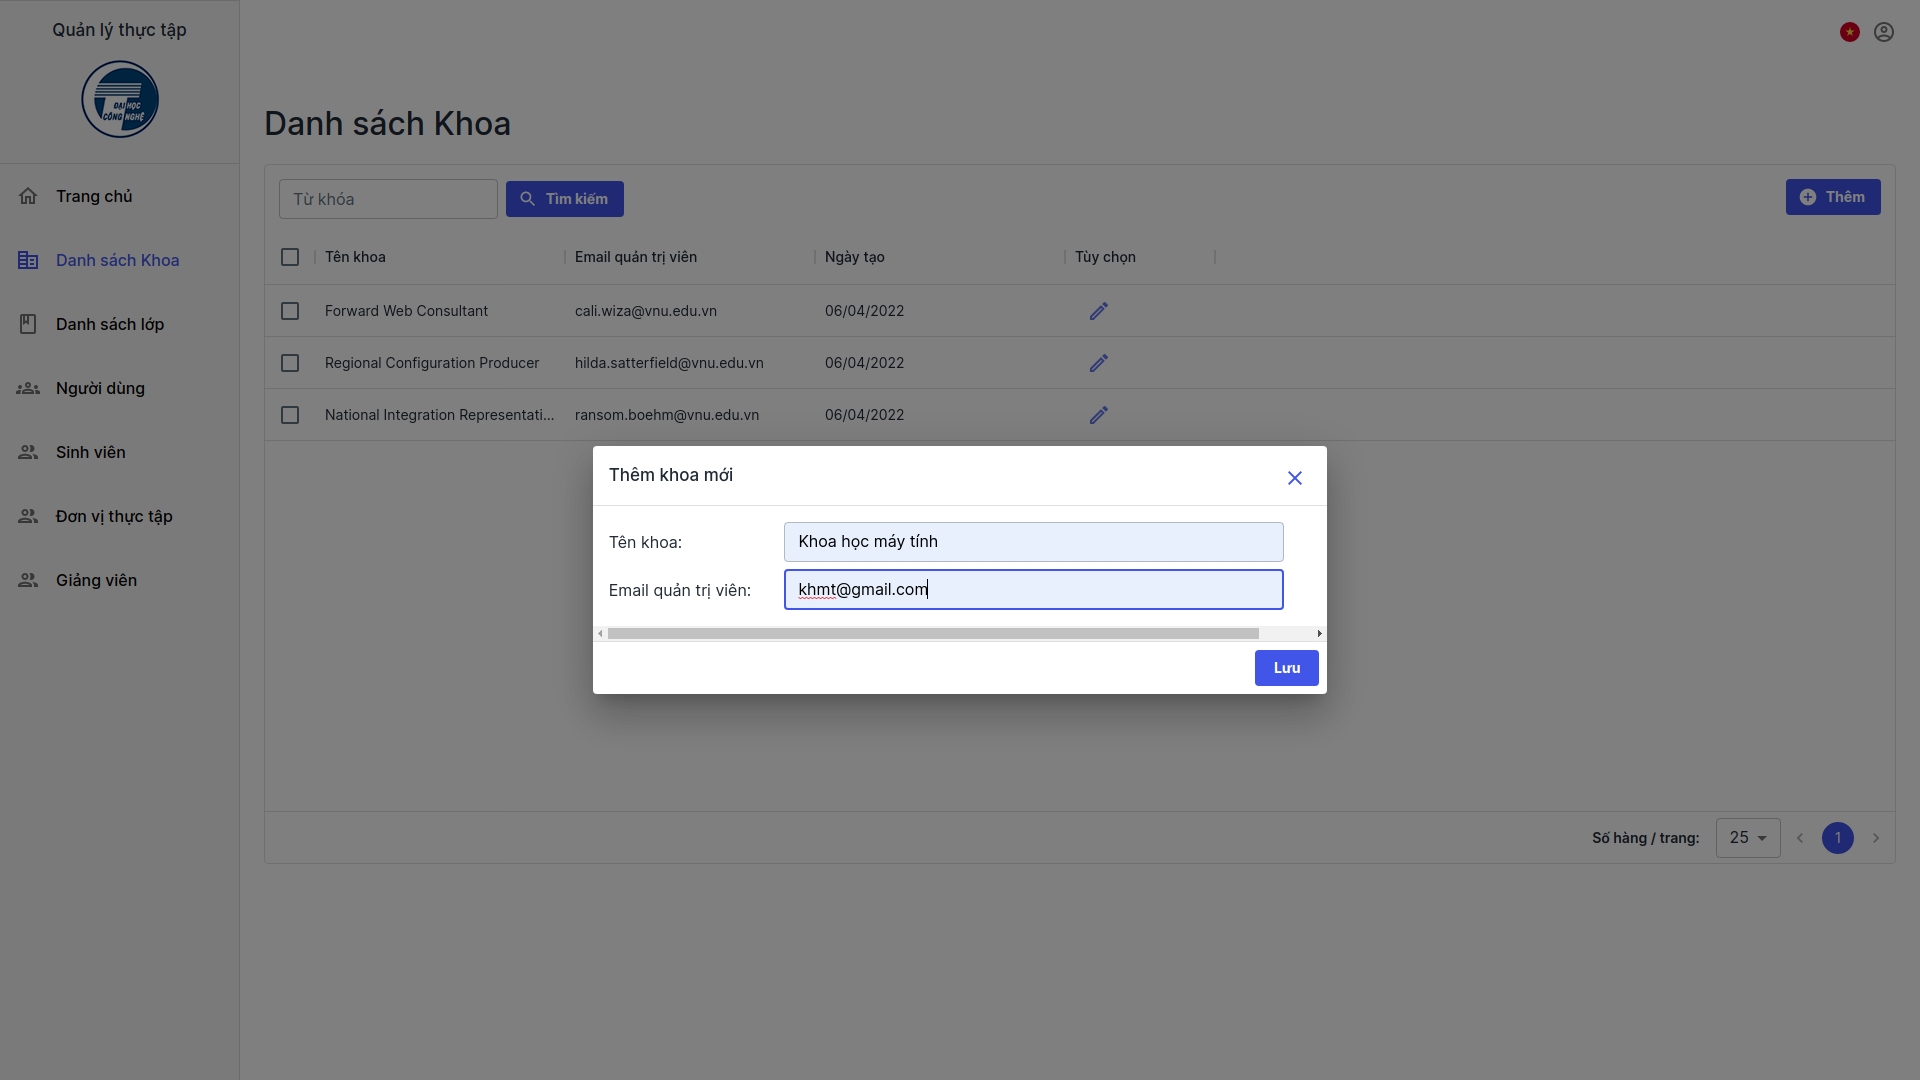
\includegraphics[width=\linewidth]{./images/image23.png} %TODO: replace image
% 	\caption{Màn hình hòm thư sau khi tạo Khoa mới thành côngg}
% 	\label{fig:add_org_success}
% \end{figure}







\end{document}